\chapter{Технологийн судалгаа}
\section{Flutter - BLoC}
"Hoome" платформын мобайл аппликейшн нь програмчлалын Dart хэл буюу Flutter технологийг ашиглан бичигдсэн бөгөөд түүн дотроо төлвийн менежмент сан болох BLoC(Business Logic Components)-ийг ашигладаг. 

BLoC нь хэрэглэгчийн интерфейсийг бизнес логикоос тусгаарлаж өгөх зорилготой сан бөгөөд event-driven архитектур дээр суурилсан байдаг. 

BLoC нь таны Flutter програмын төлвийг удирдах, хэрэглэгчийн харилцан үйлчлэлийг бүтэцтэй байдлаар зохицуулах design pattern юм. Энэ нь апп доторх data stream болон удирдахын тулд event, stream-ийн тухай ойлголтыг ашигладаг.

\subsection{Үндсэн бүтэц}

Flutter BLoC технологи нь:

\begin{enumerate}
  \item \textbf{Events}: Event нь хэрэглэгчийн аппликейшнд үзүүлэх ямарваа нэгэн хариу үйлдэл бөгөөд тухайн event-ийг BLoC компонент хүлээн авч, логик үйлдлүүдийг хийж боловсруулснаар одоо байгаа төлвүүдийг шинэчилж шинэ төлвийг үүсгэдэг.
  \item \textbf{BLoC Component}: Event-үүдийг сонсож, утга хүлээн авахад үргэлж бэлэн байдаг бөгөөд event-үүд нь өөрийн утгатай байх боломжтой. Хүлээн авсан эвентүүдийг хэрэглэгчийн интерфейст ашиглагдаж буй төлөв, төлвийн өгөгдлийг шинэчлэхэд ашигладаг.
  \item \textbf{Streams}: Event-үүд нь ихэвчлэн stream байдлаар хадгалагдаж, орсон дарааллаараа ачаалладаг бөгөөд BLoC компонентүүд нь тус бүр өөрийн зааж өгсөн урсгалыг сонсож байдаг.
  \item \textbf{States}: Аппликейшн дээр ашиглагдаж буй бүх төрлийн датаг state буюу төлөв гэж нэрэлж байгаа бөгөөд тухайн төлөв нь BLoC компонентоор дамжуулагдан шинэчлэгдэж, улмаар хэрэглэгчийн интерфейст өөрчлөлт ороход хүргэдэг. 
\end{enumerate}

Эдгээр 4 үндсэн элементүүдээс бүрдэх бөгөөд хэрэглэгчийн интерфейст шинэчлэл хийх, өөрчлөлт оруулах үед интерфесийн логикоос хамааран онцгой тохиолдол(exception), алдаа(runtime error)-наас сэргийлэх боломжтой. Аппликейшнийн usability болон scalability-г илүү амар хялбар байдлаар хангаж өгдөг сан юм. 

\begin{figure}
  \centering
  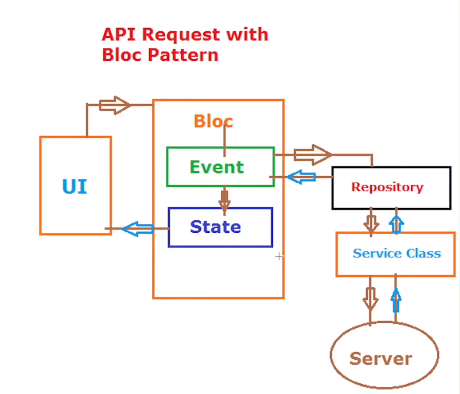
\includegraphics[scale=0.5]{imgs/bloc.png}
  \caption{BLoC }
\end{figure}

\subsection{Хэрэгжүүлэлт}

Машины дугаар бүртгэх хэсэг дээр жишээ авж үзэв.  

Хэрэглэгч машины дугаарыг бүртгүүлэх үед RegisterPlateNumber гэх event явагдах бөгөөд үүнийг onSavePlateNumber функцээр сонсож, тухайн event дээр хийгдэх бизнес логикийг бичиж өгөв. 

\begin{lstlisting}[language=Java, frame=single, caption=BLoC компонентийн машины дугаар бүртгэлийн хэрэгжүүлэлт]
import 'dart:convert';

import 'package:bloc/bloc.dart';

part 'parking_event.dart';
part 'parking_state.dart';
class ParkingBloc extends Bloc<ParkingEvent, ParkingState> {
  //... Other event handlers

  void _onSavePlateNumber(
    RegisterPlateNumber event,
    Emitter<ParkingState> emit,
  ) async {
    emit(state.copyWith(registerStatus: RegisterStatus.loading));
    bool isRegistered = await ParkingRepository().registerParking(event.phoneNumber, event.plateNumber);
    if (isRegistered) {
      LocalStorage().save('phoneNumber', event.phoneNumber, const Duration(days: 365));
      emit(state.copyWith(localPhoneNumber: event.phoneNumber));
    }

    emit(state.copyWith(
      registerStatus: isRegistered ? RegisterStatus.success : RegisterStatus.failure,
      statusMessage: 'Car registration success!',
    ));
  }
}
\end{lstlisting}

\newpage

\begin{lstlisting}[language=Java, frame=single, caption=Машины дугаарыг хэрэглэгчийн дугаарын хамтаар сервер дээр бүртгэх]
import 'package:dio/dio.dart';

class ParkingRepository {
  final Dio dio = Dio();

  //... Other repository methods

  Future<bool> registerParking(String phoneNumber, String plateNumber) async {
    final body = {
      'phoneNumber': phoneNumber,
      'plateNumber': plateNumber,
    };

    try {
      final response = await dio.post(ApiConstants.registerParkingUser, data: jsonEncode(body));
      return response.statusCode == 200 || response.statusCode == 204;
    } on DioError catch (_) {
      return false;
    }
  }
}

\end{lstlisting}
\pagebreak

\section{Spring boot - JHipster}
JHipster нь нээлттэй веб аппликейшн болон микросервисүүдийг бэлдэж өгдөг tool бөгөөд хөгжүүлэлтийн процессийг хялбарчилж, хурдлуулж өгдгөөрөө давуу талтай. Ихэвчлэн сервер талдаа Spring boot аппликейшнийг бэлдэж өгдөг бол веб дээр хэрэглэгч талдаа Angular, React зэрэг технологиудыг ашигласан бэлэн төслийг үүсгэж өгдөг.

React - Redux болон Angular дээр хөгжүүлэгчээс ямар зам (route) болон ямар authorization/authentication технологи ашиглахыг аван тохирох аппликейшнийг үүсгэж өгдөг. Энэхүү ажил нь ойролцоогоор хөгжүүлэгчийн хувьд 5-10 ажлын өдөр шаарддаг бол JHipster-ийн тусламжтайгаар төслийн төвөгтэй олон тохиргоонд цаг үрэлгүйгээр шууд үндсэн бизнес логикоо кодлох боломжийг олгодог.

Spring boot дээр ашиглахдаа authorization-ээс гадна model-оо хүртэл үүсгэж зааж өгөх боломжтой бөгөөд хөгжүүлэгч ERD-аа jdl дээр бичиж өгөн JHipster-ээр тухайн model-той холбоо бүхий бүх кодуудыг бэлдүүлэх боломжтой.

\subsection{Spring boot support}
JHipster-ийг ашиглан best practice буюу дагаж мөрдвөл хамгийн зохих, олон хөгжүүлэгчдийн санал нийлсэн байдлаар кодлосон boilerplate төслийг үүсгэх боломжтой ба 
\begin{itemize}
  \item Security - Authentication/Authorization
  \item Өгөгдлийн сангийн интеграц - JPA/Hibernate
  \item Build tools - Maven/Gradle
  \item Docker болон Kubernetes support
  \item Unit testing
\end{itemize}
зэрэг олон setup бүхий зүйлсийг хөнгөвчлөх боломжтой.

\subsection{Хэрэгжүүлэлт}
JHipster CLI ашиглан keycloak интеграц хийсэн микросервис үүсгэсэн байдал.

Энэхүү CLI коммандыг ашиглан эхний байдлаар микросервисийг үүсгэнэ.
\begin{lstlisting}[language=Bash, frame=single]
jhipster
\end{lstlisting}

\begin{lstlisting}[frame=single, caption=Keycloak realm-тай холбох Yaml тохиргоо]
spring:
security:
  oauth2:
    client:
      provider:
        oidc:
          issuer-uri: http://your-keycloak-server/auth/realms/your-realm
      registration:
        oidc:
          client-id: your-client-id
          client-secret: your-client-secret
    resource:
      userInfoUri: http://your-keycloak-server/auth/realms/your-realm/protocol/openid-connect/userinfo
\end{lstlisting}

Entity үүсгэх CLI комманд
\begin{lstlisting}[language=Bash, frame=single]
jhipster import-jdl myErd.jdl
\end{lstlisting}

Үүний дараагаар "mvnw" script файлыг үүсгэж өгөх бөгөөд микросервисийг асаахдаа 
\begin{lstlisting}[language=Bash, frame=single]
./mvnw
\end{lstlisting}

\begin{lstlisting}[language=Bash, frame=single, caption=myErd.jdl дотор буй ERD]
entity Person {
  keycloakId String,
    username String,
    firstname String,
    lastname String,
    fullname String,
    balance Integer,
    referralCode String unique,
    createdBy String,
    createdDate Instant,
    lastModifiedBy String,
    lastModifiedDate Instant,
}

entity Referral {
  keycloakId String,
    username String,
    firstname String,
    lastname String,
    fullname String,
    createdBy String,
    createdDate Instant,
}

entity PointTrans {
    amount Integer,
    transEnum TransEnum,
    description String,
    serviceEnum ServiceEnum,
    createdBy String,
    createdDate Instant,
    lastModifiedBy String,
    lastModifiedDate Instant,
}

enum TransEnum {
  INCOME, EXPENSE
}

enum ServiceEnum {
  CCP, SOH, ITSTORE, SYSTEM
}

relationship OneToMany {
  Person to Referral{person required},
    Person to PointTrans{person required},
}

skipClient *
paginate * with infinite-scroll
filter *  
\end{lstlisting}
\pagebreak
\textbf{Үр дүнд үүсэх модел болон controller-ууд}

\begin{lstlisting}[language=Java, caption=UserDTO.java, frame=single]
package mn.nomadicss.service.dto;

import mn.nomadicss.domain.User;
public class UserDTO {
    private String id;
    private String login;

    public UserDTO() {
        // Empty constructor needed for Jackson.
    }
    public UserDTO(User user) {
        this.id = user.getId();
        // Customize it here if you need, or not, firstName/lastName/etc
        this.login = user.getLogin();
    }
    public String getId() {
        return id;
    }
    public void setId(String id) {
        this.id = id;
    }
    public String getLogin() {
        return login;
    }
    public void setLogin(String login) {
        this.login = login;
    }
    @Override
    public String toString() {
        return "UserDTO{" +
            "id='" + id + '\'' +
            ", login='" + login + '\'' +
            "}";
    }
}

\end{lstlisting}
\pagebreak
\begin{lstlisting}[language=Java, caption=UserDTO.java, frame=single]
package mn.nomadicss.web.rest;
...
@RestController
@RequestMapping("/api")
public class PersonResource {
  private final Logger log = LoggerFactory.getLogger(PersonResource.class);
    private static final String ENTITY_NAME = "hoomepointPerson";

    @Value("${jhipster.clientApp.name}")
    private String applicationName;
    private final PersonService personService;
    private final PersonRepository personRepository;
    private final PersonQueryService personQueryService;

    public PersonResource(PersonService personService, PersonRepository personRepository, PersonQueryService personQueryService) {
        this.personService = personService;
        this.personRepository = personRepository;
        this.personQueryService = personQueryService;
    }

    @PostMapping("/people")
    ...
    @PutMapping("/people/{id}")
    ...
    @PatchMapping(value = "/people/{id}", consumes = { "application/json", "application/merge-patch+json" })
    ...
    @GetMapping("/people")
    ...
    //... More controllers for data access
}
\end{lstlisting}
\pagebreak
\begin{lstlisting}[language=Java, caption=UserRepository.java үүсгэсэн байдал, frame=single]
package mn.nomadicss.repository;

import java.util.List;
import java.util.Optional;
import mn.nomadicss.domain.User;
import org.springframework.data.domain.*;
import org.springframework.data.jpa.repository.EntityGraph;
import org.springframework.data.jpa.repository.JpaRepository;
import org.springframework.stereotype.Repository;

/**
 * Spring Data JPA repository for the {@link User} entity.
 */
@Repository
public interface UserRepository extends JpaRepository<User, String> {
    Optional<User> findOneByLogin(String login);

    @EntityGraph(attributePaths = "authorities")
    Optional<User> findOneWithAuthoritiesByLogin(String login);

    Page<User> findAllByIdNotNullAndActivatedIsTrue(Pageable pageable);
}
\end{lstlisting}

\textit{Цаашлаад үүсгэсэн сервисүүд болон тохиргооны файлууд, docker support файлууд, нэгжийн тестүүдийг хавсраагүй болно.}